\chapter{System Design}

Here's a picture for Chales!
There you go charles... now write some text. We believe in you!
asd
asd
asd
asd
asd

\section{Methodology}

\section{System Overview}
some text what a system overview is \\
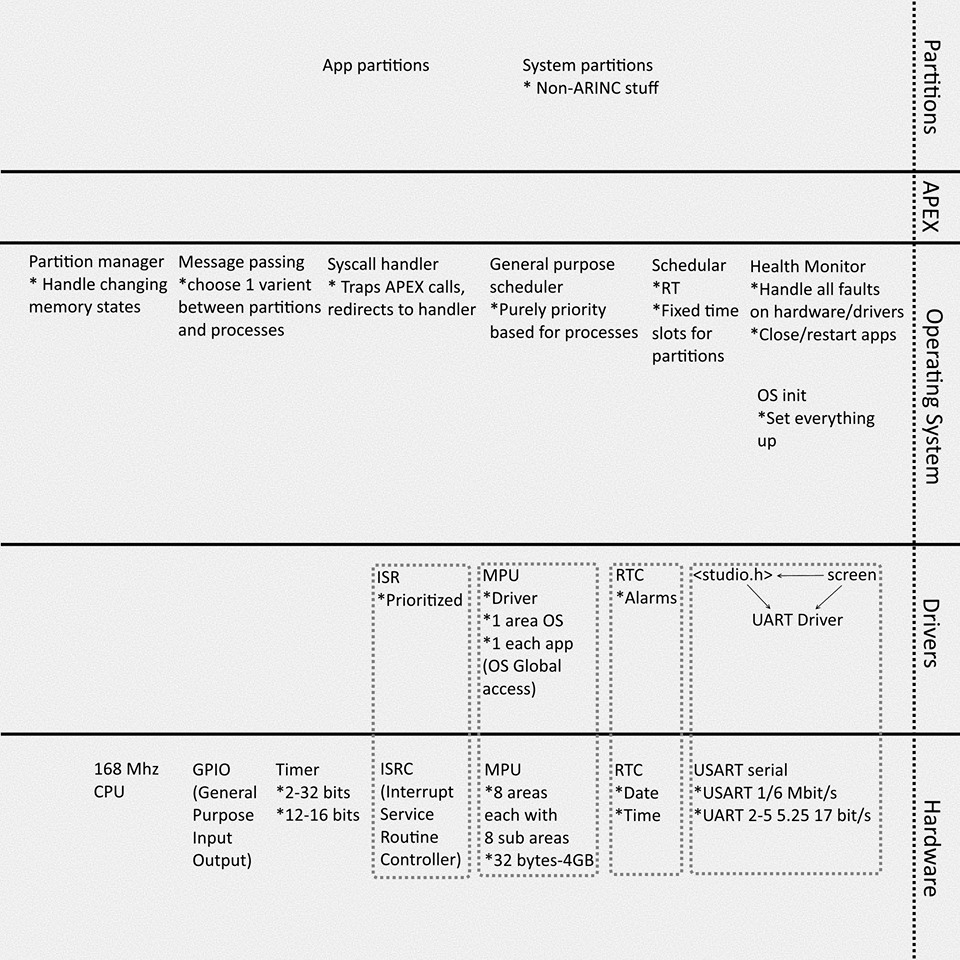
\includegraphics[width=13cm]{first_draft_sys_design_diag.jpeg}

\subsection{Layers}


\subsection{Hardware}

\subsection{Drivers}
\begin{description}[align=left]
	\item [\textbf{UART driver}] The UART is used by the system to communicate with the outside
	world. This can either receive or transmit data to another UART device.
	\item [\textbf{Watchdog timer driver}] The watchdog timer is necessary to ensure recovery
	in case of a hardware fault or program error. If this happens, the program would be restarted
	from a safe state. 
	
\end{description}

\subsection{OS}
\begin{description}[align=left]
	\item [\textbf{scheduler}] more text
	\item [\textbf{scheduler}] a whole lot of words
\end{description}
\subsubsection{Interpartition communication}

\section{XML}


\section{Memory Management}
ARINC 653 advertizes time and space seperation covered in (ref to sec in analysis).
To accommodate for the feature of seperating partitions in space
this operating system relies on the memory management unit (MPU)
to manage permissions accross sections of memory
ensuring that partitions stay within a dedicated memory space.

\subsection{something about ARINC on memory management}

\subsection{the MPU on a STM32F415}

\subsection{memory strategy}
